\documentclass{article}
%\usepackage{txfonts}
%\renewcommand*\rmdefault{ppl}
%\usepackage[utf8]{inputenc}
\usepackage{amsmath}
\usepackage{graphicx}
\usepackage{enumitem}
\usepackage{amssymb}
\usepackage{marginnote}
\newcommand{\nf}[2]{
\newcommand{#1}[1]{#2}
}
\newcommand{\nff}[2]{
\newcommand{#1}[2]{#2}
}
\newcommand{\rf}[2]{
\renewcommand{#1}[1]{#2}
}
\newcommand{\rff}[2]{
\renewcommand{#1}[2]{#2}
}

\newcommand{\nc}[2]{
  \newcommand{#1}{#2}
}
\newcommand{\rc}[2]{
  \renewcommand{#1}{#2}
}

\nff{\WTF}{#1 (\textit{#2})}

\nf{\translator}{\footnote{\textbf{Translator note:}#1}}

\newcommand{\nequ}[2]{
\begin{align*}
#1
\tag{#2}
\end{align*}
}

\newcommand{\uequ}[1]{
\begin{align*}
#1
\end{align*}
}

\newcommand{\sumXY}[2]{\underset{#1}{\overset{#2}{\sum}}}
\newcommand{\sumX}[1]{\underset{#1}{\sum}}
\newcommand{\intXY}[2]{\int_{#1}^{#2}}

\rf{\exp}{e^{#1}}

\nc{\grad}{\operatorfont{grad}}
\rc{\div}{\operatorfont{div}}

\nf{\pddt}{\frac{\partial{#1}}{\partial t}}
\nf{\ddt}{\frac{d{#1}}{dt}}

\nff{\pddX}{\frac{\partial{#1}}{\partial{#2}}}
\nc{\lap}{\Delta}
\nc{\e}{\varepsilon}

\nc{\Y}{\psi}
\nc{\y}{\varphi}

\title{Interaction of neutral atoms and homopolar binding in quantum mechanics}
\author{W. Heitler and F. London}
\date{June 30, 1927}

\begin{document}
\maketitle

\begin{abstract}
The \WTF{force}{Kr\"aftespiel} between two neutral atoms shows a characteristic quantum-mechanical \WTF{ambiguity}{Mehrdeutigkeit}. This ambiguity seems to be suitable to include the different modes of behavior provided by experiment. For e.g. hydrogen, the possibility of homopolar binding or elastic reflection, while for noble gasses only the latter - and indeed to the first approximation this already has about the right magnitude. In the selection and discussion of different behaviors the Pauli principle has also proved itself here in the application to systems of many atoms.
\end{abstract}

The theoretical treatment of the interaction between neutral atoms has up to now has caused considerable difficulty. While one has for a long time been able to make a simple model of the attractive forces bewteen ions, the behavilr of neutral atoms, in particular the possibility of a nonpolar binding, has been extraordinarily difficult to understand if one does not want to resort to very artificial explanations.

The development of quantum mechanics has however provided a new point of view for the treatment of this problem: first in the new "models" the charge distribution is of a totally different type than in the Bohr model (namely falling off as $\exp{-r}$), which would already provide an entirely different force between "neutral" atoms. More essential and decisive however for the understanding of the modes of behavior possible between neutrak atoms isa characteristically quantum-mechanical beat-phenomenon, which is closely related to the resonance-beats found by Heisenberg. We will study as an example two H-atoms (§1), as well as two He-atoms (§3). To anticipate the result (§2): one obtains two solutions for the interaction energy: one, which attracts the atoms at medium distances, yields a repulsion at short distances and which suffices for the formation of a homopolar molecule (already in the first approximation, in which perturbations due to polarization are disregarded). This solution is however not allowed for He in the ground state on the basis of the Pauli principle (§4). A second solution, which only comes into consideration for he, supplies a repulsion everywhere (van der Waals' b-force).

§1. Interaction between two hydrogen atoms.

We pose ourselves the task of determining the change in energy which two neutral ground-state hydrogen atoms experience when we bring them within a distance $R$ (measured as the distance between nuclei) of one another. Depending on whether this energy change increases or decreases through successive approximations \WTF{of the atoms}, we determine attraction or repulsion.

1. We denote the two nuclei, whose separation remains fixed at $R$ for all times, with $a$ and $b$, the two electrons with the numerals $1$ and $2$, and finally the distances of the electrons from the nuclei and from one another with $r_{a1},...,r_{12}$.

The wave equation of our problem -- the two-hydrogen-atom problem -- then reads (with $\lap_{12} = \lap_1 + \lap_2 = \frac{\partial^2}{\partial {x_1}^2} + \frac{\partial^2}{\partial {y_1}^2} + \frac{\partial^2}{\partial {z_1}^2} + \frac{\partial^2}{\partial {x_2}^2} + \frac{\partial^2}{\partial {y_2}^2} + \frac{\partial^2}{\partial {z_2}^2}$):
\nequ{
(\chi) \equiv \lap_{12}\chi + \frac{8\pi^2 m}{h^2}\left\{
E - \left(\frac{\e^2}{R} + \frac{\e^2}{r_{12}} - \frac{\e^2}{r_{a1}} - \frac{\e^2}{r_{a2}} - \frac{\e^2}{r_{b1}} - \frac{\e^2}{r_{b2}}
\right)\right\}\chi =
0.}{1}

We are interested in those solutions $\chi$, which correspond to perturbations of the two netural ground-state H-atoms, and accordingly we will approximate them by the well-known eigenfunctions of the ground state hydrogen atom.

If the electron $1$ is found at nucleus $a$, then it is assigned the well-known hydrogen eigenfunction
\nequ{
\Y(1) = \frac{1}{\sqrt{\pi}}\left(\frac{1}{a_0}\right)^\frac{3}{2}\exp{-\frac{r_{a1}}{a_0}},
}{2}
where $a_0$ denotes the Bohr radius of the $1_1$-orbit. The argument $1$ signifies the coordinates of the electron $1$ in $q$-space, in the furure we write it as an index, thus $\Y_1$ (confusion with the eigenvalue index need not be feared, since we always consider atoms in the ground state). Correspondingly,
\nequ{
\y_1 = \frac{1}{\sqrt{\pi}}\left(\frac{1}{a_0}\right)^\frac{3}{2}\exp{-\frac{r_{b1}}{a_0}},
}{2'}
means the first electron is found at the nucleus $b$. The two eigenfunctions (2) and (2') quite different, if they can be brought into alignment through a simple translation, because they are situated in different regions of space.

Corresponding eigenfunctions exist for electron $2$:
\nequ{
\Y_2 = \frac{1}{\sqrt{\pi}}\left(\frac{1}{a_0}\right)^\frac{3}{2}\exp{-\frac{r_{a2}}{a_0}},
\y_2 = \frac{1}{\sqrt{\pi}}\left(\frac{1}{a_0}\right)^\frac{3}{2}\exp{-\frac{r_{b2}}{a_0}},
}{2a}
which mean that electron $2$ is found at nucleus $a$ resp. $b$. The eigenfunctions (2a) distinguish themselves from (2) and (2') only in $q$-space.

2. We will have chosen as unperturbed eigenfunctions those which describe one electron at one nucleus and the other electron at the other nucleus. When one considers these still-uncoupled systems together as a single system, it is known that the product of these two eigenfunctions is regarded as the mutual eigenfunction. However there are two different ways of distributing the two electrons to the two nuclei. First one has
\nequ{
\Y_1 \y_2 \text{($1$ is at $a$, $2$ is at $b$)}.
}{3a}
One could just as well also have
\nequ{
\Y_2 \y_1 \text{($2$ is at $a$, $1$ is at $b$)}.
}{3b}

Both possibilities have the same total enerby (\WTF{double hydrogen energy}{doppelte Wasserstoffenergy}). There is a case of twofold degeneracy: every pair of orthogonal linear combinations of $\Y_1 \y_2$ and $\Y_2 \y_1$:
\nequ{
\alpha &= a\Y_1 \y_2 + b\Y_2
\y_1\\
\beta  &= c\Y_1 \y_2 + d\Y_2 \y_1,}{4}

with normalization and orthogonality conditions
\nequ{
a^2 + b^2 + 2abS =& 1,\\
c^2 + d^2 + 2cdS =& 1,\\
ac + bd + (ad + bc)S =& 0
}{5}
(where $S=\int\Y_1 \y_1 \Y_2 \y_2 dx_1 dx_2$) are taken as the unperturbed eigenfunctions.

3. The exact eigenfunctions of the differential equation (1) emerge from very specific linear combinations (4), the "zero-th approximation" eigenfunctions, and are distinguished from the latter only by a small perturbation $v$. The coefficients $a,b,c,d$ in (4) for these zero-th approximation eigenfunctions are determined by well-known rules. Though the equation (1) lacks the character of a perturbation problem, since one cannot treat any term in the potential function as a "perturbation potential", the method of determination of the aforentioned coefficients and the perturbation energy is exactly the same as when a perturbation potential is present. In order to make the calculation transparent, we want to choose from the outset the correct and appropriate normalized linear combinations (and their correctness will be verified later):
\nequ{
\alpha &= \frac{1}{\sqrt{2+2S}}(\Y_1\y_2 + \Y_2\y_1),\\
\beta  &= \frac{1}{\sqrt{2-2S}}(\Y_1\y_2 - \Y_2\y_1).
}{4a}
For the perturbed eigenfunctions we will now add:
\nequ{
\chi_\alpha &= \alpha + v_{\alpha}\\
\chi_\beta  &= \beta +  v_{\beta}.
}{6}
Entering this Ansatz into the equation (1) and considering that the functions $\Y_1, \Y_2, \y_1, \y_2$ to satisfy the four equations
\nequ{
\lap_1 \Y_1 &+ \frac{8\pi^2 m}{h^2}\left( E_0 + \frac{\e^2}{r_{a1}}\right)\Y_1 = 0,\\
\lap_2 \Y_2 &+ \frac{8\pi^2 m}{h^2}\left( E_0 + \frac{\e^2}{r_{a2}}\right)\Y_2 = 0,\\
\lap_1 \y_1 &+ \frac{8\pi^2 m}{h^2}\left( E_0 + \frac{\e^2}{r_{b1}}\right)\y_1 = 0,\\
\lap_2 \y_2 &+ \frac{8\pi^2 m}{h^2}\left( E_0 + \frac{\e^2}{r_{b2}}\right)\y_2 = 0,
}{7}
where $E_0 = 13.5 \text{Volts}$ denotes the eigenvalue of the hydrogen ground state. With the notation
\nequ{
E_1 = E - 2E_0
}{8}
for the perturbated eigenvalue we obtain from (1) the two differential equations for $v_\alpha$ and $b_\beta$:
\nequ{
\sqrt{2+2S}L(v_\alpha) &+ \left(E_1-\frac{\e^2}{r_{12}} - \frac{\e^2}{R}\right)(\Y_1\y_2+\Y_2\y_1)\\
&+ \left(\frac{\e^2}{r_{a1}} + \frac{\e^2}{r_{b2}}\right)\Y_2\y_1 + \left(\frac{\e^2}{r_{b1}} + \frac{\e^2}{r_{a2}}\right)\Y_1\y_2
}{9$\alpha$}
\nequ{
\sqrt{2-2S}L(v_\beta) &+ \left(E_1-\frac{\e^2}{r_{12}} - \frac{\e^2}{R}\right)(\Y_1\y_2-\Y_2\y_1)\\
&+ \left(\frac{\e^2}{r_{a1}} + \frac{\e^2}{r_{b2}}\right)\Y_2\y_1 - \left(\frac{\e^2}{r_{b1}} + \frac{\e^2}{r_{a2}}\right)\Y_1\y_2.
}{9$\beta$}

In order for these equations that are inhomogenous in $v$ for an eigenvalue $E$ the homogenous equation to be solvable at all, is to require that the inhomogenities are orthogonal to every eigenfunction of the homogenous equations which belong to the same eigenvalue $E$, thus to $\chi_\alpha$ and $\chi_\beta$.

One finds first that the inhomogenity in (9$\alpha$) is already orthogonal to $\beta$ and the inhomogenity of (9$\beta$) is orthogonal to $\alpha$ (up to ignorable values). Thus the correctness of the Ansatz (4a) is verified. The two other requirements:
\uequ{
\text{Inhomogenity (9$\alpha$)} &\perp \alpha,\\
\text{Inhomogenity (9$\beta$)} &\perp \beta,
}
supply the two perturbed eigenvalues
\nequ{
E_\alpha &= E_{11} - \frac{E_{11}S - E_{12}}{1 + S} = \frac{1}{1+S}(E_{11} + E_{12})\\
E_\beta &=  E_{11} + \frac{E_{11}S - E_{12}}{1 - S} = \frac{1}{1-S}(E_{11} - E_{12})
}{10}
with the following notation:
\nequ{
E_{11} &= \int\left[\left(\frac{\e^2}{r_{12}} + \frac{\e^2}{R} \right)
\frac{{\Y_1}^2{\y_2}^2 + {\Y_2}^2{\y_1}^2}{2} - 
\left(\frac{\e^2}{r_{a1}} + \frac{\e^2}{r_{b2}}\right)\frac{{\Y_2}^2{\y_1}^2}{2}\right] \\
&\left. -\left(\frac{\e^2}{r_{a2}} + \frac{\e^2}{r_{b1}}\right)
\frac{{\Y_1}^2{\y_2}^2}{2}\right] d\tau_1 d\tau_2,\\
E_{12} &= \int\left(\frac{2\e^2}{r_{12}} + \frac{2\e^2}{E}
 - \frac{\e^2}{r_{a1}} - \frac{\e^2}{r_{a2}} - \frac{\e^2}{r_{b1}} - \frac{\e^2}{r_{b2}}\right)
 \frac{\Y_1\y_1\Y_2\y_2}{2}d\tau_1 d\tau_2\\
S &= \int\Y_1\y_1\Y_2\y_2 d\tau_1 d\tau_2.
}{11}

§2. Discussion of the results.

1. We thus obtain two perturbation energies corresponding to the Ansatzes (5a):
\uequ{
E_\alpha = E_{11} - \frac{E_{11}S - E_{12}}{1 + S}
}
belongs to $\frac{1}{\sqrt{2 + 2S}}(\Y_1\y_2 + \Y_2\y_1)$ (symmetric in $1$ and $2$),
\uequ{
E_\beta = E_{11} - \frac{E_{11}S - E_{12}}{1 - S}
}
belongs to $\frac{1}{\sqrt{2 - 2S}}(\Y_1\y_2 - \Y_2\y_1)$ (antisymmetric in $1$ and $2$).

It is a result that can only be described with classical concepts only very artificially, that two neutral atoms can interact with eachother in two different ways. We are probably still very far away from a real understanding of this behavior. However, it is desirable to at least clarify how this remarkable ambiguity comes about mathematically. The essential thing is apparentlu that the problem is initially twofold degenerate (1a and 1b), corresponding to the two possibilities of assigning the electrons to the neutral atoms\footnote{In classical mechanics, this problem is not degenerate: the two electron assignments to indeed belong to the same eigenvalue. But the criterion for a degeneracy in classical mechanics is not $E_k - E_l = 0$, but rather $\nu \equiv \pddX{E}{J}$ (a \WTF{"neighborhood relationship"}{Nachbarschaftsbeziehung} regarding the action variable $J$). A tually, in this case the electrons also have their \WTF{full periodicity}{vollen Periodizitätsgrad}. Only when the energy is sufficient to overcome the potential barrier located between the two atoms (or to a sufficient approximation the two atoms) does $E_k-E_l=0$ have $\pddX{E}{J}$ as a consequence and the problem is degenerate. Thus the electrons now describe orbits around both nuclei and constantly exchange with eachother. In quantum mechanics this \WTF{distinction}{Fallunterscheidung} does not occur (c.f. F. Hund, ZS f. Phys. 40, 442, 1926). For ever greater (finite) potential barriers there always exists a certain corresponding probability for an exchange of the electrons. While there is a possibility in classical mechanics to label the electrons (one puts each electron in a sufficiently-deep potential well and \WTF{keeps away any larger energy inputs}{halte größere Energiezufuhr fern}), nothing corresponding is possible in quantum mechanics: if one knows that an electron is in a potential well at one instant, one is never certain whether it has not already in the next instant exchanges with another. Therefore, a statistic which disregards the principle the electrons' individuality and only considers the numerical distribution of their states, as the Bose- or Fermi-statistics, perfectly adapted to the quantum-mechanical description of possibilities.}. The resolution of this degeneracy is bouns up in, as seen in (10), to the non-vanishing of the eigenfunction of the atom $a$ at the position of the atom $b$ and vice-versa (otherwise would $\Y_1\y_1=0$ and consequently $E_{12}=0$ and $S=0$); however, that means that there must exist a finite probability for the electron of $a$ to belong to the atom $b$. The exponential behavior of $\Y$ and $\y$ actually always fulfills this requirement. The value $\frac{1}{h(E_\beta - E_\alpha)}$ is to denote the mean frequency with which an exchange of the two electrons takes place. For large distances thia difference falls off as $\frac{\e^3}{a_0}\exp{-\frac{2}{a_0}R}$, so that widely-separated atoms experience an exchange extremely seldomly.
 
This whole phenomenon is closely related with the quantum-mechanical resonance phenomena treated by Heisenberg. But while with in resonance the electrons of different \WTF{stages of movement}{Bewegungsstufen} of one and the same eigenfunction series exchange their energies, here we have electrons of the same \WTF{level of excitation}{Anregungsstufe} (same energy), but with different eigenfunction systems ($\Y$ and $\y$), exchanging their position. There the twofold occurance of the same frequency is characteristic (resonance phemonena); here on the other hand there is no talk of resonance.

2. We now turn to the qualitative discussion of the interaction energy (10). Already without evaluating the occuring integral, we can say: the sign of $E_{11}S - E_{12}$ is always positive. In a Sturm-Liouviole eigenvalue problem of arbitrarily many dimensions with homogenous boundary conditions, those eigenvibrations which have no nodes have the lowest eigenvalue. Now however the solution $\alpha$ is nodeless, while $\beta$, as an antisymmetric eigenfunction, always has a node. Thus
\nequ{
E_\beta > E_\alpha.
}{12}

The meaning of $E_{11}$ is immediately clear from (11): it is the pure Coulomb interaction of the existing charge distribution. The calculation yields
\nequ{
E_{11} = \frac{\e^2}{a_0}\exp{-\frac{2}{a_0}R}\left(
\frac{a_0}{R} + \frac{5}{8} - \frac{3}{4}\frac{R}{a_0} - \frac{1}{6}\frac{R^3}{{a_0}^3}.
\right)
}{13}
See the middle curve in figure 1. $R$ is expressed in germs of $a_0 = 0.532\AA$, the energy in volts.

The remaining part of the energy (11) cannot be so simply defined. The integrals occurring there cannot all be evaluates. One calculates
\nequ{
S &= \left(1 + \frac{R}{a_0} + \frac{R^2}{3{a_0}^2}\right)^2 \exp{-\frac{2R}{a_0}}\\
\int\frac{\Y_1\Y_2\y_1\y_2}{2} & \left(
\frac{\e^2}{r_{a1}} + \frac{\e^2}{r_{a2}} + \frac{\e^2}{r_{b1}} + \frac{\e^2}{r_{b2}} - \frac{2\e^2}{R}
\right)d\tau_1 d\tau_2\\
&= \frac{2\e^2}{a_0}\left(1 + \frac{2R}{a_0} + \frac{4}{3}\frac{R^2}{{a_0}^2} + \frac{R^3}{3{a_0}^3}\right)\exp{-\frac{2R}{a_0}} - \frac{\e^2}{R}S,
}{14}
while for the missing integral over $\frac{1}{r_{12}}$ we can only obtain an upper bound\footnote{It concerns the determination of the self-potential of a charge distribution of co-focal ellipsoids, which is very complex, like the well-known Dirichlet determination for similarly-situated ellipsoids. In the estimate (15) the ellilsoid will be replaced by a ball with the same total charge.} It is
\nequ{
\int\frac{\Y_1\Y_2\y_1\y_2}{r_{12}}d\tau_1 d\tau_2 <
\frac{\e^2}{a_0}\frac{5}{8}\left(1 + \frac{R}{a_0} + \frac{R^2}{3{a_0}^2}\right)^2 \exp{-\frac{2R}{a_0}}.
}{15}
With this upper limit, we obtain the curves $E_\alpha$ and $E_\beta$ in figure 1.

\begin{figure}[h!]
\centering
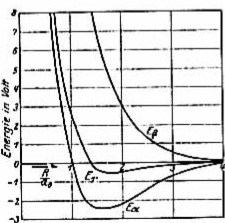
\includegraphics[width=200pt]{images/figure1}
{\caption{Potential of two neutral $H$ atoms. $E_\alpha$ = homopolar attraction, $E_\beta$ = elastic reflection.}}
\end{figure}

$E_\beta$ shows consistent repulsion; $E_\alpha$ shows an attraction at greater distances, then a minimum around $R=\frac{5}{3}a_0$\translator{Fraction barely legible}, and at smaller distances a repulsion. The nonpolar attraction occurring here shows up as a characteristically quantum-mechanical effect. It appears already without consideration of perturbations by polarisation. It is also remarkable that the repulsion $E_\beta$, as can be seen, likewise depends for the most part on this quantum-mechanical effect, and not on the Coulomb interaction.

The physical meaning of the two solutions, we assert, is the following: the antisymmetrical solution with the energy $E_\beta$ causes the van der Waals repulsion (elastic reflection) of the two hydrohgem atoms. If however $\alpha$ \WTF{is excited}{angeregt}, then the two hydrogen atoms could come together into a homopolar molecule, in which the minimum of $E_\alpha$ specifies the equilibrium position. We shall show further that in the interaction of two non-excited noble-gas atoms (§3) the solution, which would correspond to the formation of molecules, is quantum-theoretically forbidden. The basis of these assertions follows in §4.

The estimates curves give about the values of the atomic values in question: atomic diameter, dissociation energy, and moment of inertia of the molecule. As for the errors caused by the estimation, it should be notes that in every case $E_\beta$ is actually higher and $E_\alpha$ lower, so the typical character of the two potentials would come through even stronger. Since it is not our goal to calculate the numerical values as accurately as possible but rather to gain insight into the physical behavior of homopolar binding, we content ourselves with this approximation.

§3. Interaction between two $He$ atoms.

Using the same methods, we investigate the interaction between two $He$ atoms. The two nuclei are again called $a$ and $b$ and are held at a fixed distance $R$. The electrons carry the numerals $1$ through $4$. For each nucleus there is an eigenfunction, $\Y$ for the nucleus $a$, $\y$ for the nucleus $b$, which are now however each functions of two electrons, and indeed the Heisenberg $He$-theory\footnote{W. Heisenberg, ZS. f. Phys. 38, 411, 1926.} has shown that the eigenfunctions of the $He$ ground state are symmetric in the position coordinates. By forming products of a $\Y$ and a $\y$ an we produce an eigenfunction of the unperturbed problem for widely-separated neutral atoms (we again write the arguments as indices):
\nequ{
\Y_{ik}\y_{lj}\quad (i \neq k \neq l \neq j = 1,2,3,4).
}{16}
By permuting the four electrons (keeping in mind that $\Y_{ik} = \Y_{ki}, \y_{ik} = \y_{ki}$) we arrive at $\binom{4}{2} = 6$ new eigenfunctions, which all belong to the same eigenvalues. They read:
\nequ{
\Y_{12}\y_{34}, &\quad \Y_{34}\y_{12} \\
\Y_{13}\y_{42}, &\quad \Y_{42}\y_{13} \\
\Y_{14}\y_{23}, &\quad \Y_{23}\y_{14}.
}{17}
The ground-state helium electrons must differ from one another regarding their spin. We will choose the notation such that the electrons $1$ and $3$ have the same spin, likewise the electrons $2$ and $4$, but $1$ and $2$ have different spin. Then according to the Pauli principle it is forbidden that $1$ and $3$ resp. $2$ and $4$ are found at the same $He$-nucleus. We could accordingly exclude two out of the six eigenfunctions (17) and constrain ourselves to
\nequ{
\Y_{12}\y_{34}, &\quad \Y_{34}\y_{12} \\
\Y_{14}\y_{23}, &\quad \Y_{23}\y_{14}.
}{17a}
The wave equation for the $2-He$-problem reads:
\nequ{
\sumXY{i=1}{4}\left[\lap_i \chi + \frac{8\pi^2 m}{h^2}\left(E - \e^2 \left(
\frac{4}{R} + \sumXY{k=1}{4}\frac{1}{r_{ik}} - \frac{1}{r_{ai}} - \frac{1}{r_{bi}}
\right)\right)\chi \right] = 0.
}{18}

This is symmetrical in all four electrons. Here again we don't have a perturbation problem in the usual form, since there is no more a perturbation potential as in §1; we deduce from the symmetry of the differential equation that the zero-th approximation eigenfunctions are the same as if there were a small perturbation potential symmetrical in all four electrons. We denote this with $H$.

With the help of this consideration we could naturally not deduce the first-order eigenvalues of the secular problem, but probably the correct eigenfunctions of the zero-th order, if these are characterized only by the symmetry character of the differential equation. Instead, to insert the eigenfunctions (17a) into the secular problem with H, it is practical from the outset to form certain linear combinations of (17a), namely (we leave off the normalization factors):
\nequ{
\Psi_1 =
\Y_{12}\y_{34} + \Y_{34}\y_{12},& \quad \Phi_1 = \Y_{12}\y_{34} - \Y_{34}\y_{12},\\
\Psi_2 = \Y_{14}\y_{23} + \Y_{23}\y_{14},& \quad \Phi_1 = \Y_{14}\y_{23} - \Y_{23}\y_{14}.\\}{17b}


With these eigenfunctions all matrix elements of the form
\uequ{
\int H\Psi\Phi d\tau = 0,
}
vanish, because $H\Psi$ is symmetrical and $\Phi$ is antisymmetrical with respect to an exchange of $1$ and $3$ and simultaneously with $2$ and $4$; the integral is however not sensitive with respect to an exchange of the integration variables, and thus it must vanish. Furthermore the following matrix elements occur in the secular problem:
\uequ{
\int H\Psi_1^2 d\tau &= \int H\Psi_2^2 d\tau = H_{11}\\
\int H\Psi_1 \Psi_2 d\tau &= H_{13},\\
\int H\Phi_1^2 d\tau &= \int H\Phi_2^2 d\tau = K_{11}\\
\int H\Phi_1 \Phi_2 d\tau &= 0.
}

The \WTF{secular problem of the fourth degree}{Säkularproblem vierten Grades} for the perturbation energy $E$ then runs:

\begin{tabular}{l|cccc|l}
  \, & $\Psi_1$ & $\Psi_2$ & $\Phi_1$ & $\Phi_2$ \\
\hline
$\Psi_1$ & $H_{11} - E$ & $H_{12}$   & 0 & 0 \\
$\Psi_2$ & $H_{12}$     & $H_{11}-E$ & 0 & 0\\
$\Phi_1$ & 0            & 0          & $K_{11} - E$ & 0\\
$\Phi_2$ & 0            & 0          & 0 & $K_{11} - E$
\end{tabular}
= 0.

One obtains a twofold degenerate eigenvalue $K_{11}$ and two non-degenerate eigenvalues:
\nequ{
E_\alpha &= H_{11} + H_{12},\\
E_\beta  &= H_{11} - H_{12},\\
E_\gamma &= K_{11},\\
E_\delta &= K_{11}.
}{19}

Thus according to the well-known procedure one finds the eigenfunctions:
\nequ{
\alpha &= \Psi_1 + \Psi_2 = \Y_{12}\y_{34} + \Y_{34}\y_{12} + \Y_{14}\y_{23} + \Y_{23}\y{14},\\
\beta  &= \Psi_1 - \Psi_2 = \Y_{12}\y_{34} + \Y_{34}\y_{12} - \Y_{14}\y_{23} - \Y_{23}\y{14},\\
\gamma &= \Phi_1 = \Y_{12}\y_{34} - \Y_{34}\y_{12},\\
\delta &= \Phi_2 = \Y_{14}\y_{23} - \Y_{23}\y_{14}
}{20}

On the same grounds as in the 2-hydrogen problem the $E_\alpha$ must be the smallest eigenvalue, consequently $H_{12} < 0$; because to $E_\alpha$ belongs the nodeless symmetrical eigenfunction $\alpha$. We will however show in the following section that this $\alpha$, which could energetically make the formation of a molecule possible, is not quantum-mechanically allowed for neutral $He$ atoms, that rather of the four solutions (20) only $\beta$ can occur, which again means elastic reflections.

§4. The Pauli principle and molecule formation
1. As one can easily convince oneself, our solutions (4a) resp. (20) belong to systems which do not combine with one another\footnote{They are distinguished in this sense from a similar case recently investigated by F. Hund, ZS. f. Phys, 40, 742, 1927, namely the Zweizentreuproblem}. This situation opens the possibility to apply the Pauli principle, which has been proven im the discussion of the electron confogurations of the one-atom problem, in an extended sense to the system of two interacting atoms, in order to get a more accurate selection of those quantum-theoretically-allowed modes of behavior of two atoms.

The following formulation of this rule is sufficient for our purposes\footnote{This formulation of the Pauli principle is not entirely correct. However an effective generalized version of the same is unknown up to the present. We refer to Heisenberg's paper, ZS. f. Phys. 41, 239, 1927, as well as the upcoming considerations of F. Hund.}: by permuting the two electrons, the signs of the chosen eigenfunctions of the system should change resp. stay the same, if the two electrons have the same resp. different spins. (A so-called "spin eigenfunction" is not considered here.)

2. We apply this rule to the solutions of §§1 and 3. For hydrogen the symmetrical $\alpha$ maintains its sign in permuting $1$ and $2$, and in $\beta$ it changes. For $\alpha$ thus the two electrons must have different spin, and $\beta$ they must have the same spin. Since however there is no restriction on the spin of separated atoms, both solutions could occur - according to chance.

For the solutions (20) of the 2-$He$ problem however we know that $1$ and $3$ as well as $2$ and $4$ indeed do have the same spin, $1$ and $2$ as well as $3$ and $4$ on the other hand differ. The exchangability of the electrons is thus limited from the outset. If the individual $He$-atom is to remain viable (Pauli principle applied to the $He$ atom), then one may only permute the electrons $1$ with $3$ as well as $2$ with $4$. The chosen eigenfunctions must be antisymmetrical with respect to these permutations. By permuting both pairs they must again be reproduced (without sign change). The eigenfunctions $\alpha,\beta,\gamma,\delta$ now, via the named permutations, go over to: 
\begin{tabular}{l|c|c|c|c|l}
  \, & $1$ with $3$ & $2$ with $4$ & $1$ with $3$ and $2$ with $4$ \\
\hline
$\alpha \to$ & $+\alpha$ & $+\alpha$   & $+\alpha$  \\
$\beta \to$  & $-\beta$  & $-\beta$    & $+\beta$ \\
$\gamma \to$ & $-\delta$ & $+\delta$   & $-\gamma$ \\
$\delta \to$ & $-\gamma$ & $+\gamma$   & $-\delta$
\end{tabular}

We thus see that with $He$ only the solution $\beta$ satisfies the requirements. This is however associated with higher eigenvalues. If we carry over the behavior of hydrogen, then we get the upper curve $E_\beta$ from figure 1 for the dependence of the interaction on $R$, which always yields repulsion. Further discussion shows that it supplies about the right value for the $He$-radius according to the kinetic theory of gas. The additional restriction which we found here for $He$, clearly has its basis in the fact that two $He$-atoms (and the same applies for all noble gasses) can not be distinguished with respect to their spin -- in contradistinction to hydrogen (and all atoms with unfilled shells) --, whereby two $He$-atoms only a single mode of behavior is possible.

3. We now wish to show which of these \WTF{distinguished}{ausgeschiedeben} solutions permit the formation of a molecule. The following characterization of a molecule seems to be correct for a wide class of cases\footnote{In this regard we lean on the considerations of H.G. Grimm and A. Sommerfeld, ZS. f. Phys. 36, 36, 1926, as well as Hund, l.c.}: the configuration of those electrons which take part in the binding of the molecule, should be adiabatically transferrable (i.e. without quantum jumps) into a configuration allowed by the Pauli principle.

One sees immediately, the solution $\alpha$ of hydrogen is in this sense capable of forming a molecule\footnote{They naturally don't necessarily lead to the formation of a molecule. Whether that occurs depends on the initial conditions.}: by adiabatically moving the nuclei towards one another the ground state of the $He$-atom ($1^1 S$) would result. $E_\alpha$ actually shows (figure 1) a strong attraction, -- the equilibrium position corresponds to the normal position of the $H_2$ molecule.

The solution $\beta$ of hydrogen occurs, as we see, when the two electrons have the same spin. In the transferral to an $He$-type state, two equivalent orbits with the same spin would result. This is however excluded [this would be the lowest state of the triplet system ($1^3 S$), which is not available, and which has played so great a role in the discovery of the Pauli principle]. $\beta$ can thus not lead to molecule formation -- and as the so-to-say guardian of the Pauli principle we see a considerable repulsion would prohibit any approach\translator{verb illegible}.

The solutions $\alpha,\beta,\gamma,\delta$ could never lead to an molecule formation, because there would then be four electrons in a $K$-shell, which is however excluded. However it would be quite possible to form a viable shell with excited $He$-atoms, which would give several reciprocal modes of behavior, according to the available spin, and it is in this sense that one may understand the existence of very unstable $He_2$ molecules, among others.

4. The considerations of the previous section will appear to be incomplete as long as it is not shown that the attractive force, which leads to the formation of homopolar molecules, dies out as soon as the available chemical valence is saturated.

One easily sees that between two systems, which regarding their electron spins can only be oriented with respect to one another only in one manner, only one eigenvibration of the type $\beta$ can exist (as we have seen e.g. with $He$), which has a node, and as a consequence here one will expect it to always have, as with $He$, a repulsion. This is clearly already the case when the system has at least one closed shell configuration, thus e.g. $H_2 + H$, $He + H$, $H_2 + H_2$, etc. Additionally, the impossibility of forming $H_3-$, $H_4-$, $HeH-$ molecules from unexcited atoms already emerges from the limited space in the $K$-shell.

§5. Hydrogen and ion formation.

Our considerations in the first sections could not be complete, insofar as the possibility of ion formation has not been taken into account. \WTF{There we had taken as our Ansatz the results of the functions (3)}{Wir hätten dort in unseren Ansätzen den Ausgang genommen von den Funktionen (3)}:
\uequ{
\Y_1 \y_2 \text{ resp. } \y_1 \Y_2,
}
which assigns one electron to each nucleus, -- corresponding to our question as to the interaction of neutral atoms.

If we are now interested in the interaction between two $H$ ions ($H^+$ and $H^-$), we will have to consider the configurations with two electrons at the same nucleus:
\nequ{
\Y_1\Y_2 \text{ resp. } \y_1\y_2,
}{21}
which we have taken into account up to now. -- One might think that this omission was incorrect, since the eigenfunctions (21) belong to the same eigenvalue \WTF{as the (3) we been using exclusively up to now, that we had thus started from a four-fold degeneracy}{wie die von uns bisher allein benutzten (3), daß wir also von einer vierfachen Entartung auszugehen hätten}.

This is however not correct: even for far-separated ions, the very considerable perturbations of the two electrons on eachother are taken into account from the outset if both electrons are located at the same nucleus (analogous to perturbations in the $He$-atom). We obtain for the separate ions instead of the $2E_0$ ($-27$ volts) of neutral atoms a higher energy around the work of ionization ($13.5$ volts - adjusted by the electron affinity, which is very insignificant). Correspondingly instead of using (21) as eigenfunctions, $He$-type perturbed functions are used:
\uequ{
\Y_{12} \text{ resp. } \y_{12},
}
which are always symmetrical in $1$ and $2$ and only differ in the position in the $q$-space, not in the form.

If we now consider the perturbation of the $He$-type ion $H^{-}$ by $H^{+}$, then we obtain, because of the symmetry character of the wave equation (1), the zero-th order eigenfunctions (without normalization) in the usual manner:
\nequ{
\alpha^* &= \Y_{12} + \y_{12},\\
\beta^*  &= \Y_{12} - \y_{12}.
}{22}

By mutual approach of the two ions, the associated eigenvalues $E_\alpha^*$ and $E_\beta^*$ will first decrease approximately as the ionization potential $-\frac{\e^2}{R}$ (figure 2). Thus will $E_\alpha^*$, belonging to the node-free $\alpha^*$, always be lower than $E_\beta^*$. The difference $E_\beta^* - E_\alpha^*$ is proportional to the frequency of exchange of the ion-charge.

\begin{figure}[h!]
\centering
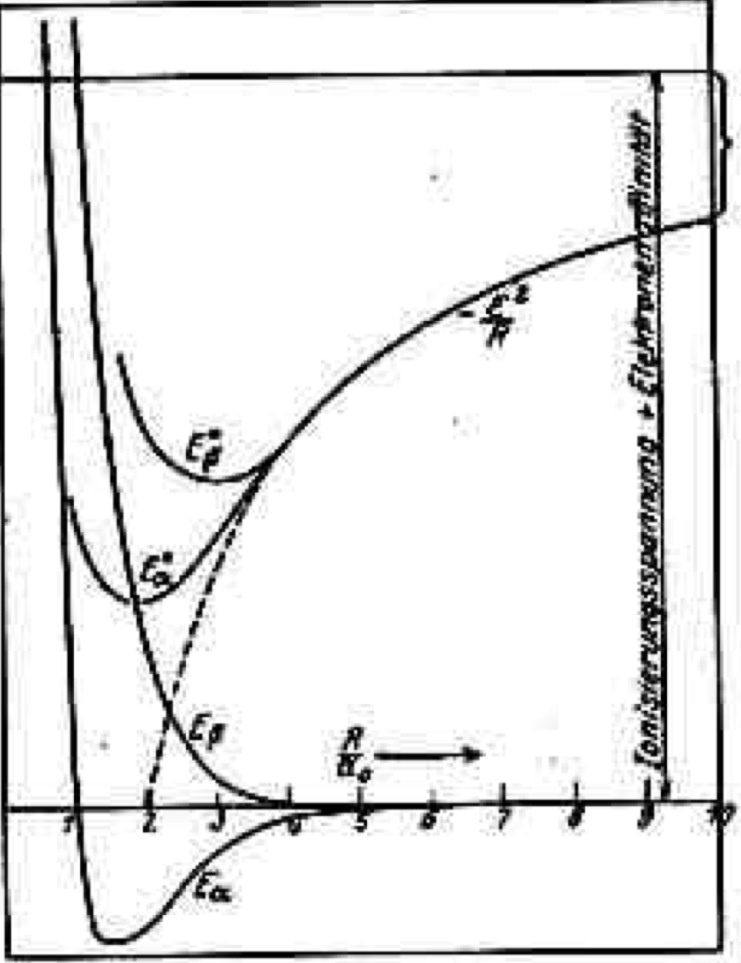
\includegraphics[width=200pt]{images/figure2}
{\caption{Ionization potential ($E_\alpha^*$, $E_\beta^*$)} comparison with the potential of neutral atoms ($E_\alpha$, $E_\beta$)}
\end{figure}

So long as the eigenvalues $E_\alpha^*$ and $E_\beta^*$ don't come into the vicinity of our energy curves from §2 (they are drawn once again in figure 2), the calculations of §1 are interpreted as perturbations of the eigenvalues $2E_0 = -27$ volt and are not to be complained about. Something new occurs, however, when the new curves come very near to the old ones. \WTF{For these values of $R$ the eigenfunctions in question become degenerate, the "correct" zero-th order eigenfunctions then become certain linear combinations of the eigenfunctions at the intersection, which result from a secular problem}{Für diese Werte von R wird der betreffende Eigenwert mehrfach, man hat Entartung, die "richtigen" Eigenfunktionen nullter Ordnung werden dann gewisse Linearkombinationen der Eigenfunktionen vor dem Schnittpunkt, welche sich durch ein Säkularproblem ergeben.}. The calculations of §1 would thus be problematic if in this situation different linear combinations arose than those used there. We shall now prove this:

1. \WTF{$E_\beta$ will be intersected by the higher of the two energy curves - first $E_\alpha^*$, and eventually $E_\beta^*$}{Zuerst werden $E_\alpha^*$ und eventuell $E_\beta^*$ die obere der beiden Energiekurven $E_\beta$ schneiden}. Since $\alpha^*$ and $\beta^*$ are symmetrical while $\beta$ is antisymmetrical in $1$ and $2$, and this symmetry behavior is not lost even with arbitrarily-large perturbations because of the symmetry of the differential equation in $1$ and $2$, the matrix elements of the "perturbation energy"\footnote{On this function $H$, see §3.} $H$ which occur in the secular problem vanish:
\uequ{
\int H\alpha^* \beta d\tau_1 d\tau_2 &= 0,\\
\int H\beta^* \beta d\tau_1 d\tau_2  &= 0.
}

The secular problem of the intersection point of $E_\alpha^*$ with $E_\beta$ thus reads:

\begin{tabular}{|cc|}
  $\int H{\alpha^*}^2 d\tau - E$ & $0$ \\
  $0$ & $\int H\beta^2 d\tau - E$
\end{tabular} = 0.

One obtains an equivalent secular problem for the intersection of $E_\beta^*$ with $E_\beta$. From this emerges that the secular eigenvalues are the same as the original, and further, that the eigenfunctions come through unmixed, without forming linear combinations\footnote{One can view this \WTF{unmixingness}{Unvermengbarkeit} of $\beta$ with $\alpha^*$ and $\beta^*$ physically, since $\beta$ has parallel spins, and $\alpha^*$ and $\beta^*$ (namely the symmetric $He$-ground state configuration) have different spins; if the configuration $\beta$ exists between two atoms, it cannot thus at the same time be $\alpha^*$ or $\beta^*$. A linear combination of $\beta$ with $\alpha^*$ or $\beta^*$ would be totally incomprehensible.}.

2. \WTF{Then $\alpha^*$ and $\alpha$ will have to be dealt with}{Sodann wird $\alpha^*$ sich mit $\alpha$ ausdinanderzusetzen haben}. If one would only take the ionization potential to be $\frac{-\e^2}{R}$, then $E_\alpha^*$ would intersect the $x$-axis at $R=2a_0$ (fig. 2, dotted curve). In this region however one is already noticeably inside the charge cloud (it is essentially as large for $H^-$ as for $H$), and consequently in there the ion-attraction will gradually cease and a repulsion will take its place\footnote{The availability of an ion-repulsion for smaller distances (on the basis of the quantum-mechanical charge distribution) has already been noted independently by L. Pauling, Proc. Roy. Soc. (A) 114, 181, 1927, and A. Unsold, ZS. f. Phys. (at press).}. It is easily seen that even considering the exchange terms the two curves $E_\alpha^*$ and $E_\alpha$ in the neighborhood of the minimum of $E_\alpha$ still remain apart (figure 2, the extended curve $E_\alpha^*$ is only qualitative). The linear combination of $\alpha$ and $\alpha^*$ will accordingly still be weak in the neighborhood of $R=2a_0$ - one could interpret it as a perturbation of the eigenfunction $\alpha$. It will on this account be valid to calculate $E_\alpha$ without consideration of the linear combinations with $E_\alpha^*$, and precisely in this way is the molecule characterized as "\WTF{mainly}{vorwiegende} homopolar". For its part, $E_\alpha^*$ likewise has a minimum; at this position there would thus be room for a polar molecule. However, insofar as this minimum is not a global minimum, and insofar as it can be taken over adiabatically\footnote{The word "adiabatic" somewhat out of place here, since the transition \WTF{passes by a point of degeneracy}{durch einem Pu kte der Entartung hindurchgeht}.} to our well-known absolute minimum, one would be correct im saying that the polar molecule does not represent the stable configuration of the two $H$-atoms in the molecule. By separating the molecules without simultaneously exciting them, one would thus expect with greater probability to find two neutral atoms. In what manmer the two solutions $\alpha$ and $\alpha^*$ (linearly) combine cannot be determined without deeper invetsigation.

\WTF{The solution $\beta^*$ (antisymmetric in $\Y$ and $\y$) would eventually come through the solution $\alpha$ undisturbed on the basis of tbe same considerations as above}{Die Lösung $\beta^*$ schließlich (antisymmetrisch in $\Y$ und $\y$) würde ungestört die Lösung $\alpha$ auf Grund derselben Überlegungen wie oben durchsetzen}. Persumably however it won't come to that. In molecule formation $\beta^*$ doea not come into consideration because of its non-transferability into a $He$-configuration - it has a node between the nuclei.

We would like to believe that the categories of degeneracy and symmetry behavior discovered here could be typical for a wide range of circumstances, which are related to the interactions of atomic systems on one another, above all with the discontinuities of thekr chemical modes of behavior\footnote{One will see whether the exchange phenomena, which is so decisive for the interactions between atoms, makes itself usefuk in other areas of physics. We would like to make tw points here. In the collision processes the exchange of collision and atomic electrons brings with it the possibility of stimulating quantum jumps between \WTF{apparently}{optisch} non-combining term-systems (e.g. $1^1S - 2^3S$ in $He$). According to the Born theory such transitions are only possible on the basis of the minimal magnetic interaction. In the interpretatoon of the force-laws of the atomic nucleus, which are manifested in the scattering experiments with $\alpha$- or $H$-particles, one will have to take into acdount the exchange of nuclear constituents as an essential influence.}

We would like to give hearty thanks to Herrn Prof. Schr\"odinger for the interest which he has shown in our work. We thank the International Education Board, which has made it possible for us to work here in Zurich.

Zurich, Physikal. Institut der Universität, June 1927.





\end{document}
